\documentclass[leqno]{article}
\usepackage[utf8]{inputenc}
\usepackage{enumitem}
\usepackage{tikz}
\usepackage[parfill]{parskip} % Don't start new paragraph with tab.
\usepackage{amsmath} % For \tag and \eqref

\title{Computationele logica}
\author{
    Kamans, Jim\\
    \texttt{10302905}
    \and
    Roosingh, Sander\\
    \texttt{11983957}
    \and
    Schenk, Stefan\\
    \texttt{11881798}
}
\date{November 2017}

\begin{document}

\maketitle


%%%%%%%%%%%%%%%%
%% Exercise 1 %%
%%%%%%%%%%%%%%%%
\section{Exercise 1}

\begin{enumerate}

    \item The sentence $\theta$ encoding all information: \\

    The Queen knows the following: \\
    Alice knows Bob has a red hat. Alice knows Bob doesn't know it, and she
    knows the Queen knows this. Alice doesn't know her own hat. \\
    Bob knows Alice has a red hat. Bob knows Alice doesn't know it, and he
    knows the Queen knows this. Bob doesn't know his own hat. \\

    $\theta$ =
        $K_q (
        K_a (
            r_b \wedge
            \neg K_b (r_b \vee w_b) \wedge
            K_q ((r_a \vee r_w) \wedge (r_b \vee r_w))
        )
        \wedge \neg K_a (r_a \vee w_a)
        \wedge
        K_b (
            r_a \wedge
            \neg K_a (r_a \vee w_a) \wedge
            K_q ((r_a \vee r_w) \wedge (r_b \vee r_w))
        )
        \wedge \neg K_b (r_b \vee w_b)
        )$

    \item A representation of the situation model \textbf{M}: \\

    $\mathcal{A}$ = \{a, b, q\} the agents Alice, Bob, and the Queen \\
    $\Phi$ = $\{r_a, w_a, r_b, w_b\}$ written as WR for:
    a is white and b is red \\

    \begin{center}
    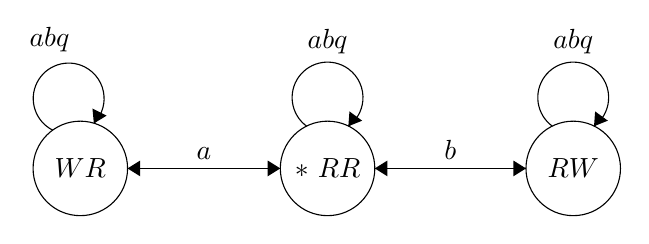
\begin{tikzpicture}[scale=0.2]
    \tikzstyle{every node}+=[inner sep=0pt]
    \draw [black] (38.4,-13.7) circle (3);
    \draw (38.4,-13.7) node {$*\mbox{ }RR$};
    \draw [black] (54,-13.7) circle (3);
    \draw (54,-13.7) node {$RW$};
    \draw [black] (22.7,-13.7) circle (3);
    \draw (22.7,-13.7) node {$WR$};
    \draw [black] (41.4,-13.7) -- (51,-13.7);
    \fill [black] (51,-13.7) -- (50.2,-13.2) -- (50.2,-14.2);
    \draw (46.2,-13.2) node [above] {$b$};
    \draw [black] (51,-13.7) -- (41.4,-13.7);
    \fill [black] (41.4,-13.7) -- (42.2,-14.2) -- (42.2,-13.2);
    \draw [black] (35.4,-13.7) -- (25.7,-13.7);
    \fill [black] (25.7,-13.7) -- (26.5,-14.2) -- (26.5,-13.2);
    \draw (30.55,-13.2) node [above] {$a$};
    \draw [black] (25.7,-13.7) -- (35.4,-13.7);
    \fill [black] (35.4,-13.7) -- (34.6,-13.2) -- (34.6,-14.2);
    \draw [black] (37.077,-11.02) arc (234:-54:2.25);
    \draw (38.4,-6.45) node [above] {$abq$};
    \fill [black] (39.72,-11.02) -- (40.6,-10.67) -- (39.79,-10.08);
    \draw [black] (52.677,-11.02) arc (234:-54:2.25);
    \draw (54,-6.45) node [above] {$abq$};
    \fill [black] (55.32,-11.02) -- (56.2,-10.67) -- (55.39,-10.08);
    \draw [black] (20.955,-11.274) arc (243.46232:-44.53768:2.25);
    \draw (20.74,-6.36) node [above] {$abq$};
    \fill [black] (23.56,-10.84) -- (24.37,-10.35) -- (23.47,-9.9);
    \end{tikzpicture}
    \end{center}

    This is an epistemic model: YES \\

    \pagebreak

    \item Seperately a and b look in their mirrors and see their red hats, the
    queen sees everything, represented in the event model $\Sigma$ with four
    actions: \\

    \begin{center}
    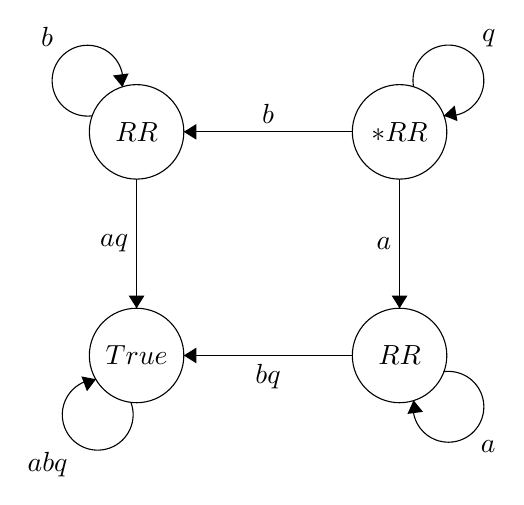
\begin{tikzpicture}[scale=0.2]
    \tikzstyle{every node}+=[inner sep=0pt]
    \draw [black] (54,-42.2) circle (3);
    \draw (54,-42.2) node {$RR$};
    \draw [black] (37.3,-28) circle (3);
    \draw (37.3,-28) node {$RR$};
    \draw [black] (37.3,-42.2) circle (3);
    \draw (37.3,-42.2) node {$True$};
    \draw [black] (54,-28) circle (3);
    \draw (54,-28) node {$*RR$};
    \draw [black] (56.805,-43.229) arc (97.58097:-190.41903:2.25);
    \draw (59.62,-47.57) node [below] {$a$};
    \fill [black] (54.89,-45.05) -- (54.5,-45.91) -- (55.49,-45.78);
    \draw [black] (34.491,-26.979) arc (277.76012:-10.23988:2.25);
    \draw (31.61,-22.64) node [above] {$b$};
    \fill [black] (36.4,-25.15) -- (36.79,-24.29) -- (35.8,-24.42);
    \draw [black] (51,-42.2) -- (40.3,-42.2);
    \fill [black] (40.3,-42.2) -- (41.1,-42.7) -- (41.1,-41.7);
    \draw (45.65,-42.7) node [below] {$bq$};
    \draw [black] (37.3,-31) -- (37.3,-39.2);
    \fill [black] (37.3,-39.2) -- (37.8,-38.4) -- (36.8,-38.4);
    \draw (36.8,-35.1) node [left] {$aq$};
    \draw [black] (51,-28) -- (40.3,-28);
    \fill [black] (40.3,-28) -- (41.1,-28.5) -- (41.1,-27.5);
    \draw (45.65,-27.5) node [above] {$b$};
    \draw [black] (54,-31) -- (54,-39.2);
    \fill [black] (54,-39.2) -- (54.5,-38.4) -- (53.5,-38.4);
    \draw (53.5,-35.1) node [left] {$a$};
    \draw [black] (54.889,-25.147) arc (190.43418:-97.56582:2.25);
    \draw (59.67,-22.63) node [above] {$q$};
    \fill [black] (56.81,-26.97) -- (57.68,-27.32) -- (57.5,-26.33);
    \draw [black] (36.935,-45.166) arc (20.7166:-267.2834:2.25);
    \draw (31.65,-48.34) node [below] {$abq$};
    \fill [black] (34.72,-43.71) -- (33.8,-43.53) -- (34.15,-44.47);
    \end{tikzpicture}
    \end{center}

    This is an epistemic model: NO \\
    This is a doxasic model: YES \\

    \item The update product of the two models \textbf{M}
    $\bigotimes$ $\Sigma$ : \\

    \begin{center}
    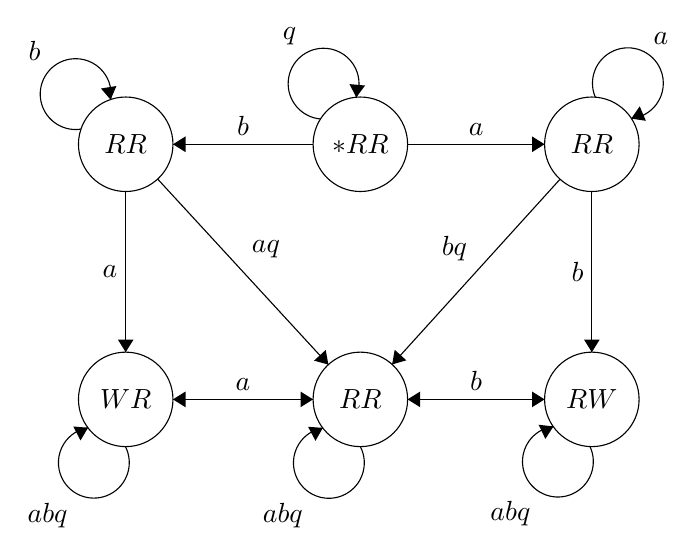
\begin{tikzpicture}[scale=0.2]
    \tikzstyle{every node}+=[inner sep=0pt]
    \draw [black] (8.5,-48.9) circle (3);
    \draw (8.5,-48.9) node {$WR$};
    \draw [black] (23.4,-48.9) circle (3);
    \draw (23.4,-48.9) node {$RR$};
    \draw [black] (38.1,-48.9) circle (3);
    \draw (38.1,-48.9) node {$RW$};
    \draw [black] (8.5,-32.7) circle (3);
    \draw (8.5,-32.7) node {$RR$};
    \draw [black] (23.4,-32.7) circle (3);
    \draw (23.4,-32.7) node {$*RR$};
    \draw [black] (38.1,-32.7) circle (3);
    \draw (38.1,-32.7) node {$RR$};
    \draw [black] (8.476,-51.888) arc (27.27123:-260.72877:2.25);
    \draw (3.54,-55.44) node [below] {$abq$};
    \fill [black] (6.11,-50.7) -- (5.17,-50.62) -- (5.63,-51.51);
    \draw [black] (23.394,-51.888) arc (27.62144:-260.37856:2.25);
    \draw (18.48,-55.46) node [below] {$abq$};
    \fill [black] (21.02,-50.71) -- (20.08,-50.64) -- (20.55,-51.53);
    \draw [black] (37.977,-51.886) arc (25.36938:-262.63062:2.25);
    \draw (32.93,-55.33) node [below] {$abq$};
    \fill [black] (35.66,-50.62) -- (34.72,-50.51) -- (35.15,-51.41);
    \draw [black] (26.4,-48.9) -- (35.1,-48.9);
    \fill [black] (35.1,-48.9) -- (34.3,-48.4) -- (34.3,-49.4);
    \draw (30.75,-48.4) node [above] {$b$};
    \draw [black] (20.4,-48.9) -- (11.5,-48.9);
    \fill [black] (11.5,-48.9) -- (12.3,-49.4) -- (12.3,-48.4);
    \draw (15.95,-48.4) node [above] {$a$};
    \draw [black] (11.5,-48.9) -- (20.4,-48.9);
    \fill [black] (20.4,-48.9) -- (19.6,-48.4) -- (19.6,-49.4);
    \draw [black] (35.1,-48.9) -- (26.4,-48.9);
    \fill [black] (26.4,-48.9) -- (27.2,-49.4) -- (27.2,-48.4);
    \draw [black] (8.5,-35.7) -- (8.5,-45.9);
    \fill [black] (8.5,-45.9) -- (9,-45.1) -- (8,-45.1);
    \draw (8,-40.8) node [left] {$a$};
    \draw [black] (5.671,-31.737) arc (278.9367:-9.0633:2.25);
    \draw (2.71,-27.44) node [above] {$b$};
    \fill [black] (7.54,-29.87) -- (7.91,-29) -- (6.93,-29.16);
    \draw [black] (20.4,-32.7) -- (11.5,-32.7);
    \fill [black] (11.5,-32.7) -- (12.3,-33.2) -- (12.3,-32.2);
    \draw (15.95,-32.2) node [above] {$b$};
    \draw [black] (20.879,-31.095) arc (265.25323:-22.74677:2.25);
    \draw (18.9,-26.43) node [above] {$q$};
    \fill [black] (23.14,-29.72) -- (23.7,-28.97) -- (22.71,-28.88);
    \draw [black] (26.4,-32.7) -- (35.1,-32.7);
    \fill [black] (35.1,-32.7) -- (34.3,-32.2) -- (34.3,-33.2);
    \draw (30.75,-32.2) node [above] {$a$};
    \draw [black] (38.325,-29.72) arc (203.42077:-84.57923:2.25);
    \draw (42.48,-26.39) node [above] {$a$};
    \fill [black] (40.6,-31.07) -- (41.53,-31.21) -- (41.14,-30.29);
    \draw [black] (38.1,-35.7) -- (38.1,-45.9);
    \fill [black] (38.1,-45.9) -- (38.6,-45.1) -- (37.6,-45.1);
    \draw (37.6,-40.8) node [left] {$b$};
    \draw [black] (10.53,-34.91) -- (21.37,-46.69);
    \fill [black] (21.37,-46.69) -- (21.2,-45.76) -- (20.46,-46.44);
    \draw (16.48,-39.34) node [right] {$aq$};
    \draw [black] (36.08,-34.92) -- (25.42,-46.68);
    \fill [black] (25.42,-46.68) -- (26.32,-46.42) -- (25.58,-45.75);
    \draw (30.21,-39.34) node [left] {$bq$};
    \end{tikzpicture}
    \end{center}

    This is an epistemic model: NO \\
    This is a doxasic model: YES \\

\end{enumerate}


%%%%%%%%%%%%%%%%
%% Exercise 2 %%
%%%%%%%%%%%%%%%%
\section{Exercise 2}

\begin{enumerate}

    \item Representation of the bits world as an epistemic model \textbf{M}: \\

    \begin{center}
    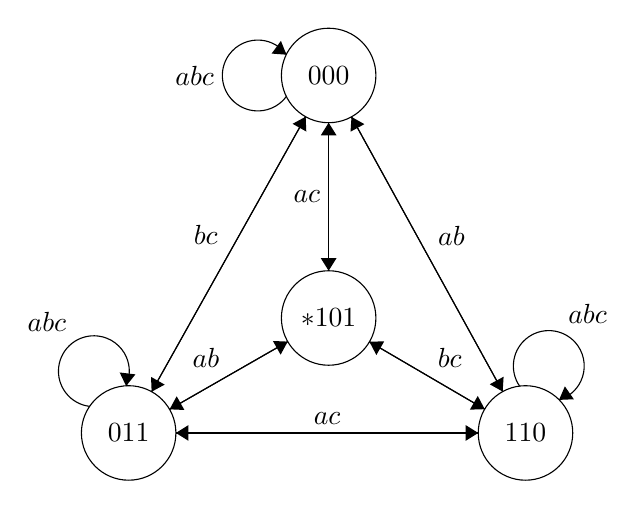
\begin{tikzpicture}[scale=0.2]
    \tikzstyle{every node}+=[inner sep=0pt]
    \draw [black] (40.3,-10.1) circle (3);
    \draw (40.3,-10.1) node {$000$};
    \draw [black] (27.6,-32.8) circle (3);
    \draw (27.6,-32.8) node {$011$};
    \draw [black] (52.8,-32.8) circle (3);
    \draw (52.8,-32.8) node {$110$};
    \draw [black] (40.3,-25.5) circle (3);
    \draw (40.3,-25.5) node {$*101$};
    \draw [black] (29.06,-30.18) -- (38.84,-12.72);
    \fill [black] (38.84,-12.72) -- (38.01,-13.17) -- (38.88,-13.66);
    \draw [black] (40.3,-22.5) -- (40.3,-13.1);
    \fill [black] (40.3,-13.1) -- (39.8,-13.9) -- (40.8,-13.9);
    \draw [black] (40.3,-13.1) -- (40.3,-22.5);
    \fill [black] (40.3,-22.5) -- (40.8,-21.7) -- (39.8,-21.7);
    \draw (39.8,-17.8) node [left] {$ac$};
    \draw [black] (30.2,-31.3) -- (37.7,-27);
    \fill [black] (37.7,-27) -- (36.76,-26.96) -- (37.25,-27.83);
    \draw [black] (37.7,-27) -- (30.2,-31.3);
    \fill [black] (30.2,-31.3) -- (31.14,-31.34) -- (30.65,-30.47);
    \draw (32.51,-28.65) node [above] {$ab$};
    \draw [black] (41.75,-12.73) -- (51.35,-30.17);
    \fill [black] (51.35,-30.17) -- (51.41,-29.23) -- (50.53,-29.71);
    \draw [black] (51.35,-30.17) -- (41.75,-12.73);
    \fill [black] (41.75,-12.73) -- (41.69,-13.67) -- (42.57,-13.19);
    \draw (47.22,-20.26) node [right] {$ab$};
    \draw [black] (42.89,-27.01) -- (50.21,-31.29);
    \fill [black] (50.21,-31.29) -- (49.77,-30.45) -- (49.27,-31.32);
    \draw [black] (50.21,-31.29) -- (42.89,-27.01);
    \fill [black] (42.89,-27.01) -- (43.33,-27.85) -- (43.83,-26.98);
    \draw (47.99,-28.65) node [above] {$bc$};
    \draw [black] (30.6,-32.8) -- (49.8,-32.8);
    \fill [black] (49.8,-32.8) -- (49,-32.3) -- (49,-33.3);
    \draw [black] (49.8,-32.8) -- (30.6,-32.8);
    \fill [black] (30.6,-32.8) -- (31.4,-33.3) -- (31.4,-32.3);
    \draw (40.2,-32.3) node [above] {$ac$};
    \draw [black] (38.84,-12.72) -- (29.06,-30.18);
    \fill [black] (29.06,-30.18) -- (29.89,-29.73) -- (29.02,-29.24);
    \draw (33.29,-20.24) node [left] {$bc$};
    \draw [black] (37.62,-11.423) arc (324:36:2.25);
    \draw (33.05,-10.1) node [left] {$abc$};
    \fill [black] (37.62,-8.78) -- (37.27,-7.9) -- (36.68,-8.71);
    \draw [black] (25.133,-31.114) arc (263.38389:-24.61611:2.25);
    \draw (22.41,-26.42) node [above] {$abc$};
    \fill [black] (27.44,-29.82) -- (28.03,-29.08) -- (27.03,-28.96);
    \draw [black] (52.432,-29.834) arc (214.79929:-73.20071:2.25);
    \draw (56.74,-25.87) node [above] {$abc$};
    \fill [black] (54.93,-30.7) -- (55.87,-30.66) -- (55.3,-29.84);
    \end{tikzpicture}
    \end{center}

    \item Representation of event model $\Sigma$:

    \begin{center}
    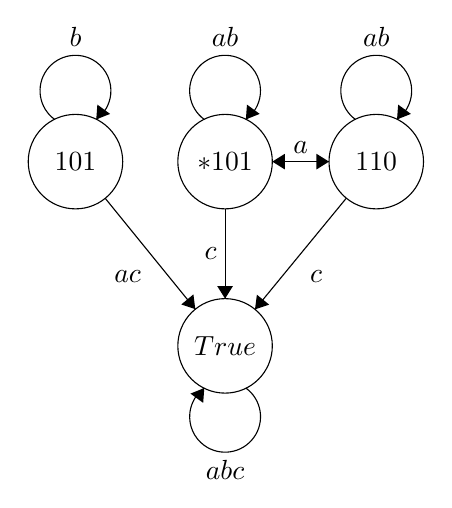
\begin{tikzpicture}[scale=0.2]
    \tikzstyle{every node}+=[inner sep=0pt]
    \draw [black] (9.4,-37.3) circle (3);
    \draw (9.4,-37.3) node {$101$};
    \draw [black] (18.9,-37.3) circle (3);
    \draw (18.9,-37.3) node {$*101$};
    \draw [black] (28.5,-37.3) circle (3);
    \draw (28.5,-37.3) node {$110$};
    \draw [black] (18.9,-49) circle (3);
    \draw (18.9,-49) node {$True$};
    \draw [black] (8.077,-34.62) arc (234:-54:2.25);
    \draw (9.4,-30.05) node [above] {$b$};
    \fill [black] (10.72,-34.62) -- (11.6,-34.27) -- (10.79,-33.68);
    \draw [black] (17.577,-34.62) arc (234:-54:2.25);
    \draw (18.9,-30.05) node [above] {$ab$};
    \fill [black] (20.22,-34.62) -- (21.1,-34.27) -- (20.29,-33.68);
    \draw [black] (27.177,-34.62) arc (234:-54:2.25);
    \draw (28.5,-30.05) node [above] {$ab$};
    \fill [black] (29.82,-34.62) -- (30.7,-34.27) -- (29.89,-33.68);
    \draw [black] (25.5,-37.3) -- (21.9,-37.3);
    \fill [black] (21.9,-37.3) -- (22.7,-37.8) -- (22.7,-36.8);
    \draw (23.7,-36.8) node [above] {$a$};
    \draw [black] (11.29,-39.63) -- (17.01,-46.67);
    \fill [black] (17.01,-46.67) -- (16.89,-45.73) -- (16.12,-46.37);
    \draw (13.59,-44.58) node [left] {$ac$};
    \draw [black] (20.223,-51.68) arc (54:-234:2.25);
    \draw (18.9,-56.25) node [below] {$abc$};
    \fill [black] (17.58,-51.68) -- (16.7,-52.03) -- (17.51,-52.62);
    \draw [black] (26.6,-39.62) -- (20.8,-46.68);
    \fill [black] (20.8,-46.68) -- (21.7,-46.38) -- (20.92,-45.75);
    \draw (24.26,-44.58) node [right] {$c$};
    \draw [black] (18.9,-40.3) -- (18.9,-46);
    \fill [black] (18.9,-46) -- (19.4,-45.2) -- (18.4,-45.2);
    \draw (18.4,-43.15) node [left] {$c$};
    \draw [black] (21.9,-37.3) -- (25.5,-37.3);
    \fill [black] (25.5,-37.3) -- (24.7,-36.8) -- (24.7,-37.8);
    \end{tikzpicture}
    \end{center}

    \pagebreak
    \item Representation of model \textbf{M'}:

    \begin{center}
    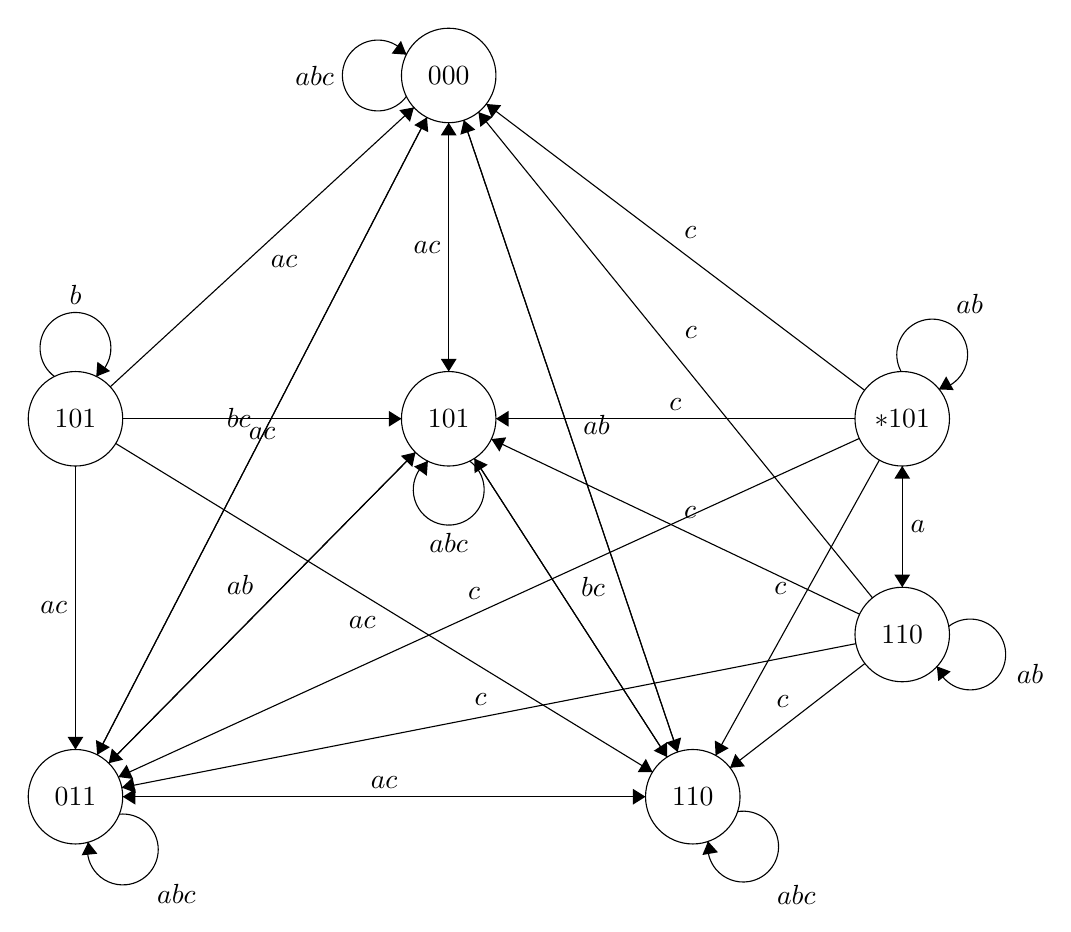
\begin{tikzpicture}[scale=0.2]
    \tikzstyle{every node}+=[inner sep=0pt]
    \draw [black] (32.1,-3.4) circle (3);
    \draw (32.1,-3.4) node {$000$};
    \draw [black] (8.4,-49.2) circle (3);
    \draw (8.4,-49.2) node {$011$};
    \draw [black] (47.6,-49.2) circle (3);
    \draw (47.6,-49.2) node {$110$};
    \draw [black] (32.1,-25.2) circle (3);
    \draw (32.1,-25.2) node {$101$};
    \draw [black] (60.9,-25.2) circle (3);
    \draw (60.9,-25.2) node {$*101$};
    \draw [black] (60.9,-38.9) circle (3);
    \draw (60.9,-38.9) node {$110$};
    \draw [black] (8.4,-25.2) circle (3);
    \draw (8.4,-25.2) node {$101$};
    \draw [black] (9.78,-46.54) -- (30.72,-6.06);
    \fill [black] (30.72,-6.06) -- (29.91,-6.55) -- (30.8,-7);
    \draw [black] (32.1,-22.2) -- (32.1,-6.4);
    \fill [black] (32.1,-6.4) -- (31.6,-7.2) -- (32.6,-7.2);
    \draw [black] (32.1,-6.4) -- (32.1,-22.2);
    \fill [black] (32.1,-22.2) -- (32.6,-21.4) -- (31.6,-21.4);
    \draw (31.6,-14.3) node [left] {$ac$};
    \draw [black] (10.51,-47.07) -- (29.99,-27.33);
    \fill [black] (29.99,-27.33) -- (29.07,-27.55) -- (29.79,-28.26);
    \draw [black] (29.99,-27.33) -- (10.51,-47.07);
    \fill [black] (10.51,-47.07) -- (11.43,-46.85) -- (10.71,-46.14);
    \draw (19.73,-35.73) node [left] {$ab$};
    \draw [black] (33.06,-6.24) -- (46.64,-46.36);
    \fill [black] (46.64,-46.36) -- (46.86,-45.44) -- (45.91,-45.76);
    \draw [black] (46.64,-46.36) -- (33.06,-6.24);
    \fill [black] (33.06,-6.24) -- (32.84,-7.16) -- (33.79,-6.84);
    \draw (40.61,-25.58) node [right] {$ab$};
    \draw [black] (33.73,-27.72) -- (45.97,-46.68);
    \fill [black] (45.97,-46.68) -- (45.96,-45.74) -- (45.12,-46.28);
    \draw [black] (45.97,-46.68) -- (33.73,-27.72);
    \fill [black] (33.73,-27.72) -- (33.74,-28.66) -- (34.58,-28.12);
    \draw (40.47,-35.89) node [right] {$bc$};
    \draw [black] (11.4,-49.2) -- (44.6,-49.2);
    \fill [black] (44.6,-49.2) -- (43.8,-48.7) -- (43.8,-49.7);
    \draw [black] (44.6,-49.2) -- (11.4,-49.2);
    \fill [black] (11.4,-49.2) -- (12.2,-49.7) -- (12.2,-48.7);
    \draw (28,-48.7) node [above] {$ac$};
    \draw [black] (30.72,-6.06) -- (9.78,-46.54);
    \fill [black] (9.78,-46.54) -- (10.59,-46.05) -- (9.7,-45.6);
    \draw (19.56,-25.16) node [left] {$bc$};
    \draw [black] (29.42,-4.723) arc (324:36:2.25);
    \draw (24.85,-3.4) node [left] {$abc$};
    \fill [black] (29.42,-2.08) -- (29.07,-1.2) -- (28.48,-2.01);
    \draw [black] (11.174,-50.311) arc (95.90564:-192.09436:2.25);
    \draw (14.81,-54.71) node [below] {$abc$};
    \fill [black] (9.21,-52.08) -- (8.79,-52.92) -- (9.79,-52.82);
    \draw [black] (50.435,-50.146) arc (99.2849:-188.7151:2.25);
    \draw (52.92,-55.42) node [right] {$abc$};
    \fill [black] (48.57,-52.03) -- (48.21,-52.9) -- (49.2,-52.73);
    \draw [black] (60.835,-22.212) arc (208.98311:-79.01689:2.25);
    \draw (65.18,-18.57) node [above] {$ab$};
    \fill [black] (63.23,-23.33) -- (64.17,-23.38) -- (63.69,-22.51);
    \draw [black] (63.844,-38.386) arc (127.63752:-160.36248:2.25);
    \draw (68.14,-41.39) node [right] {$ab$};
    \fill [black] (63.1,-40.92) -- (63.19,-41.86) -- (63.98,-41.25);
    \draw [black] (7.077,-22.52) arc (234:-54:2.25);
    \draw (8.4,-17.95) node [above] {$b$};
    \fill [black] (9.72,-22.52) -- (10.6,-22.17) -- (9.79,-21.58);
    \draw [black] (8.4,-28.2) -- (8.4,-46.2);
    \fill [black] (8.4,-46.2) -- (8.9,-45.4) -- (7.9,-45.4);
    \draw (7.9,-37.2) node [left] {$ac$};
    \draw [black] (10.61,-23.17) -- (29.89,-5.43);
    \fill [black] (29.89,-5.43) -- (28.96,-5.6) -- (29.64,-6.34);
    \draw (21.65,-14.79) node [below] {$ac$};
    \draw [black] (11.4,-25.2) -- (29.1,-25.2);
    \fill [black] (29.1,-25.2) -- (28.3,-24.7) -- (28.3,-25.7);
    \draw (20.25,-25.7) node [below] {$ac$};
    \draw [black] (10.96,-26.77) -- (45.04,-47.63);
    \fill [black] (45.04,-47.63) -- (44.62,-46.79) -- (44.1,-47.64);
    \draw (26.61,-37.7) node [below] {$ac$};
    \draw [black] (60.9,-35.9) -- (60.9,-28.2);
    \fill [black] (60.9,-28.2) -- (60.4,-29) -- (61.4,-29);
    \draw (61.4,-32.05) node [right] {$a$};
    \draw [black] (60.9,-28.2) -- (60.9,-35.9);
    \fill [black] (60.9,-35.9) -- (61.4,-35.1) -- (60.4,-35.1);
    \draw [black] (58.53,-40.74) -- (49.97,-47.36);
    \fill [black] (49.97,-47.36) -- (50.91,-47.27) -- (50.3,-46.48);
    \draw (53.3,-43.55) node [above] {$c$};
    \draw [black] (58.19,-37.61) -- (34.81,-26.49);
    \fill [black] (34.81,-26.49) -- (35.32,-27.28) -- (35.75,-26.38);
    \draw (47.43,-31.54) node [above] {$c$};
    \draw [black] (57.96,-39.48) -- (11.34,-48.62);
    \fill [black] (11.34,-48.62) -- (12.23,-48.96) -- (12.03,-47.98);
    \draw (34.13,-43.47) node [above] {$c$};
    \draw [black] (58.17,-26.45) -- (11.13,-47.95);
    \fill [black] (11.13,-47.95) -- (12.06,-48.07) -- (11.65,-47.17);
    \draw (33.72,-36.69) node [above] {$c$};
    \draw [black] (59.01,-36.57) -- (33.99,-5.73);
    \fill [black] (33.99,-5.73) -- (34.11,-6.67) -- (34.88,-6.04);
    \draw (47.06,-19.72) node [right] {$c$};
    \draw [black] (58.51,-23.39) -- (34.49,-5.21);
    \fill [black] (34.49,-5.21) -- (34.83,-6.09) -- (35.43,-5.29);
    \draw (47.45,-13.8) node [above] {$c$};
    \draw [black] (57.9,-25.2) -- (35.1,-25.2);
    \fill [black] (35.1,-25.2) -- (35.9,-25.7) -- (35.9,-24.7);
    \draw (46.5,-24.7) node [above] {$c$};
    \draw [black] (59.45,-27.82) -- (49.05,-46.58);
    \fill [black] (49.05,-46.58) -- (49.88,-46.12) -- (49,-45.63);
    \draw (53.58,-36) node [left] {$c$};
    \draw [black] (33.423,-27.88) arc (54:-234:2.25);
    \draw (32.1,-32.45) node [below] {$abc$};
    \fill [black] (30.78,-27.88) -- (29.9,-28.23) -- (30.71,-28.82);
    \end{tikzpicture}
    \end{center}



    \item Representation of event model \textbf{$\Sigma$'}:

    \item The update product of the two models \textbf{M''} = \textbf{M}
    $\bigotimes$ \textbf{$\Sigma$'} : \\

\end{enumerate}


%%%%%%%%%%%%%%%%
%% Exercise 3 %%
%%%%%%%%%%%%%%%%
\section{Exercise 3}

\begin{enumerate}

    \item \textit{How many possible worlds} are there (that are consistent with the story above)?\\
    \begin{center}
    	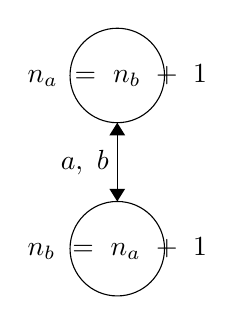
\begin{tikzpicture}[scale=0.2]
    	\tikzstyle{every node}+=[inner sep=0pt]
    	\draw [black] (44,-12.6) circle (3);
    	\draw (44,-12.6) node {$n_{a}\mbox{ }=\mbox{ }n_{b}\mbox{ }+\mbox{ }1$};
    	\draw [black] (44,-23.6) circle (3);
    	\draw (44,-23.6) node {$n_{b}\mbox{ }=\mbox{ }n_{a}\mbox{ }+\mbox{ }1$};
    	\draw [black] (44,-15.6) -- (44,-20.6);
    	\fill [black] (44,-20.6) -- (44.5,-19.8) -- (43.5,-19.8);
    	\draw (43.5,-18.1) node [left] {$a,\mbox{ }b$};
    	\draw [black] (44,-20.6) -- (44,-15.6);
    	\fill [black] (44,-15.6) -- (43.5,-16.4) -- (44.5,-16.4);
    	\end{tikzpicture}
    \end{center}
    
    \item Represent (draw) the above situation as an epistemic model M1, with two agents (a for Alice, b for Bob),  using pairs of numbers (na,nb) as “names” for the possible worlds. Draw the epistemic accessibility  relations for each agent. but  do
    not worry about the valuation (yet), since no atomic sentences are given yet.\\
    \begin{center}
    	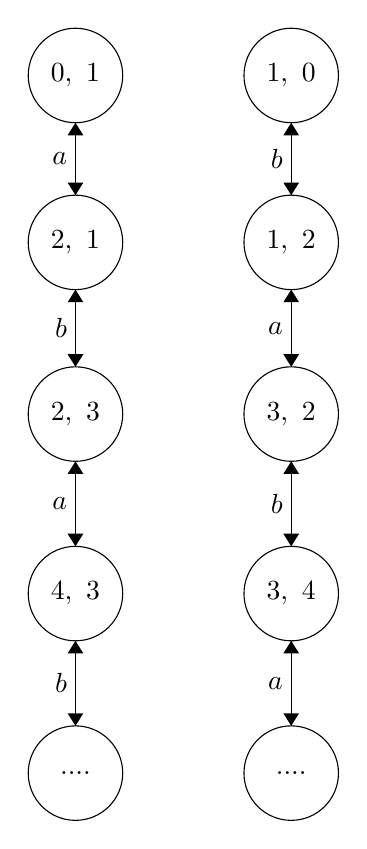
\begin{tikzpicture}[scale=0.2]
    	\tikzstyle{every node}+=[inner sep=0pt]
    	\draw [black] (25,-11.7) circle (3);
    	\draw (25,-11.7) node {$0,\mbox{ }1$};
    	\draw [black] (38.7,-11.7) circle (3);
    	\draw (38.7,-11.7) node {$1,\mbox{ }0$};
    	\draw [black] (38.7,-22.3) circle (3);
    	\draw (38.7,-22.3) node {$1,\mbox{ }2$};
    	\draw [black] (25,-22.3) circle (3);
    	\draw (25,-22.3) node {$2,\mbox{ }1$};
    	\draw [black] (25,-33.2) circle (3);
    	\draw (25,-33.2) node {$2,\mbox{ }3$};
    	\draw [black] (38.7,-33.2) circle (3);
    	\draw (38.7,-33.2) node {$3,\mbox{ }2$};
    	\draw [black] (25,-44.6) circle (3);
    	\draw (25,-44.6) node {$4,\mbox{ }3$};
    	\draw [black] (38.7,-44.6) circle (3);
    	\draw (38.7,-44.6) node {$3,\mbox{ }4$};
    	\draw [black] (25,-56) circle (3);
    	\draw (25,-56) node {$....$};
    	\draw [black] (38.7,-56) circle (3);
    	\draw (38.7,-56) node {$....$};
    	\draw [black] (25,-14.7) -- (25,-19.3);
    	\fill [black] (25,-19.3) -- (25.5,-18.5) -- (24.5,-18.5);
    	\draw (24.5,-17) node [left] {$a$};
    	\draw [black] (38.7,-14.7) -- (38.7,-19.3);
    	\fill [black] (38.7,-19.3) -- (39.2,-18.5) -- (38.2,-18.5);
    	\draw (38.2,-17) node [left] {$b$};
    	\draw [black] (38.7,-25.3) -- (38.7,-30.2);
    	\fill [black] (38.7,-30.2) -- (39.2,-29.4) -- (38.2,-29.4);
    	\draw (38.2,-27.75) node [left] {$a$};
    	\draw [black] (25,-25.3) -- (25,-30.2);
    	\fill [black] (25,-30.2) -- (25.5,-29.4) -- (24.5,-29.4);
    	\draw (24.5,-27.75) node [left] {$b$};
    	\draw [black] (38.7,-36.2) -- (38.7,-41.6);
    	\fill [black] (38.7,-41.6) -- (39.2,-40.8) -- (38.2,-40.8);
    	\draw (38.2,-38.9) node [left] {$b$};
    	\draw [black] (38.7,-47.6) -- (38.7,-53);
    	\fill [black] (38.7,-53) -- (39.2,-52.2) -- (38.2,-52.2);
    	\draw (38.2,-50.3) node [left] {$a$};
    	\draw [black] (25,-47.6) -- (25,-53);
    	\fill [black] (25,-53) -- (25.5,-52.2) -- (24.5,-52.2);
    	\draw (24.5,-50.3) node [left] {$b$};
    	\draw [black] (25,-36.2) -- (25,-41.6);
    	\fill [black] (25,-41.6) -- (25.5,-40.8) -- (24.5,-40.8);
    	\draw (24.5,-38.9) node [left] {$a$};
    	\draw [black] (25,-19.3) -- (25,-14.7);
    	\fill [black] (25,-14.7) -- (24.5,-15.5) -- (25.5,-15.5);
    	\draw [black] (38.7,-19.3) -- (38.7,-14.7);
    	\fill [black] (38.7,-14.7) -- (38.2,-15.5) -- (39.2,-15.5);
    	\draw [black] (38.7,-30.2) -- (38.7,-25.3);
    	\fill [black] (38.7,-25.3) -- (38.2,-26.1) -- (39.2,-26.1);
    	\draw [black] (25,-30.2) -- (25,-25.3);
    	\fill [black] (25,-25.3) -- (24.5,-26.1) -- (25.5,-26.1);
    	\draw [black] (25,-41.6) -- (25,-36.2);
    	\fill [black] (25,-36.2) -- (24.5,-37) -- (25.5,-37);
    	\draw [black] (38.7,-41.6) -- (38.7,-36.2);
    	\fill [black] (38.7,-36.2) -- (38.2,-37) -- (39.2,-37);
    	\draw [black] (38.7,-53) -- (38.7,-47.6);
    	\fill [black] (38.7,-47.6) -- (38.2,-48.4) -- (39.2,-48.4);
    	\draw [black] (25,-53) -- (25,-47.6);
    	\fill [black] (25,-47.6) -- (24.5,-48.4) -- (25.5,-48.4);
    	\end{tikzpicture}
    \end{center}
    \item
    \item
    \item
    \item
    \item
    \item
    \item

\end{enumerate}


\end{document}


